%%%%%解析几何模版%%%%%
\chapter*{解析几何每日一题}

\refer{《高等数学》同济版}

\exercise{
    证明以下向量相关的结论：

    \begin{enumerate}
        \item $\vv{a}\times\vv{b}=-\vv{b}\times\vv{a}$
        \item $\qty(\vv{a}+\vv{b})\times\vv{c}=\vv{a}\times\vv{c}+\vv{b}\times\vv{c}$
        \item $\qty(\lambda\vv{a})\times\vv{b}=\vv{a}\times\qty(\lambda\vv{b})=\lambda\qty(\vv{a}\times\vv{b})$，其中$\lambda$为常数
    \end{enumerate}
}
\teacher{张浈瑞}

\postdate{2023年4月16日}

\result{\mbox{相见下述证明过程}}

\begin{enumerate}
    \item 证明：$\vv{a}\times\vv{b}=-\vv{b}\times\vv{a}$
 
    \analysis{利用外积的定义进行验证即可，但需要注意，可以选取右手定则以逆时针的方向为正方向，这样根据最终的符号就可以判断方向，算出来\color{red}{\textbf{正就是}}\color{black}与正方向一致，算出来
    负则与正方向相反.
    \begin{center}
        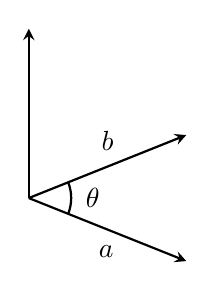
\begin{tikzpicture}
            \draw [thick,-stealth] (0,0)--(0,2.15);
            \draw [thick,-stealth] (0,0)--(2,-0.8);
            \draw [thick,-stealth] (0,0)--(2,0.8);
            \draw [thick] (0.5,-0.2) arc (-21.8:21.8:0.539);
            \node [anchor=west] at (0.6,0) {$\theta$};
            \node [anchor=north east] at (1.2,-0.48) {$\vv{a}$};
            \node [anchor=south east] at (1.2,0.48) {$\vv{b}$};
        \end{tikzpicture}
    \end{center}
    }

    \proof{
        根据定义我们可得左式：
        \formula{\vv{a}\times\vv{b}=\abs{\vv{a}}\abs{\vv{b}}\sin{\theta}}
        同时右式也可由定义得
        \formula{\vv{b}\times\vv{a}=\abs{\vv{b}}\abs{\vv{a}}\sin{\theta}}
        即证：$\vv{b}\times\vv{a}=-\vv{a}\times\vv{b}$
    }
    \item 证明：$\qty(\vv{a}+\vv{b})\times\vv{c}=\vv{a}\times\vv{c}+\vv{b}\times\vv{c}$
    \analysis{依旧从定义出发，由于方向显然是相同的，主要考虑大小，而外积的大小是以两向量为边的平行四边形的面积，从而考虑画图作垂线，从几何关系上来解决.}


    在证明过程中，可以同第一问一样通过符号同时对方向和大小进行证明.
    \proof{
        \begin{center}
            \begin{tikzpicture}[scale=0.6]
                \coordinate [label=left:{$A$}] (A) at (0,1.31);
                \coordinate [label=below right:{$B$}] (B) at (10.72,0);
                \coordinate [label=above left:{$C$}] (C) at (1.21,4.53);
                \coordinate [label=above right:{$D$}] (D) at (11.94,3.23);
                \coordinate [label=above right:{$E$}] (E) at (7.6,8.11);
                \coordinate [label=above left:{$F$}] (F) at (4.02,4.91);
                \coordinate [label=above left:{$G$}] (G) at (6.55,7.18);
                \coordinate [label=right:{$H$}] (H) at (2.53,3.57);
                \coordinate [label=right:{$I$}] (I) at (13.3,2.27);
                \draw [gray,ultra thick,-stealth] (A)--(B)node[black,midway,anchor=north]{$\vv{b}$};
                \draw [gray,ultra thick,-stealth] (B)--(D);
                \draw [gray,ultra thick,-stealth] (C)--(D);
                \draw [gray,ultra thick,-stealth] (A)--(C)node[black,midway,anchor=east]{$\vv{a}$};
                \draw [red!60!blue!75!,ultra thick,-stealth] (A)--(D)node[black,midway,anchor=north]{$\vv{a}+\vv{b}$};
                \draw [red!75!blue!60!,ultra thick] (A)--(F);
                \draw [red!75!blue!60!,ultra thick] (F)--(G)node[black,midway,anchor=south east]{$\vv{c}$};
                \draw [red!75!blue!60!,ultra thick] (G)--(E);
                \draw [gray,ultra thick] (C)--(H);
                \draw [gray,ultra thick] (F)--(B)--(I)--(G);
                \shade[ball color=darkgray] (A) circle (0.12);
                \shade[ball color=darkgray] (B) circle (0.12);
                \shade[ball color=darkgray] (C) circle (0.12);
                \shade[ball color=darkgray] (D) circle (0.12);
                \shade[ball color=darkgray] (E) circle (0.12);
                \shade[ball color=darkgray] (F) circle (0.12);
                \shade[ball color=darkgray] (G) circle (0.12);
                \shade[ball color=darkgray] (H) circle (0.12);
                \shade[ball color=darkgray] (I) circle (0.12);
                \pic["$\alpha$", draw=red!80!green!60!, <->, >=stealth, ultra thick, angle eccentricity=1.15, angle radius=35]{angle=E--A--C};
                \pic["$\alpha$", draw=red!80!green!60!, <->, >=stealth, ultra thick, angle eccentricity=1.15, angle radius=35]{angle=I--B--D};
                \pic["$\beta$", draw=green!80!red!60!, <->, >=stealth, ultra thick, angle eccentricity=1.15, angle radius=50]{angle=B--A--E};
                \pic["$\theta$", draw=blue!80!red!60!, <->, >=stealth, ultra thick, angle eccentricity=1.15, angle radius=70]{angle=D--A--E};
            \end{tikzpicture}
        \end{center}

    做$BL//AG$，又因为$BD//AC$

    则易证
    \formula{\triangle ACH\cong\triangle BDI\mbox{，四边形}BIGF\mbox{为矩形}}
    则有
    \formula{DI=CH}
    那么有
    \formula{
        \addtolength{\jot}{-1em}
        \begin{aligned}
            \qty(\vv{a}+\vv{b})\times\vv{c}&=\abs{DG}\abs{AG}=\abs{BF-DL}\abs{AG}\\
            &=\abs{BF-CH}\abs{AG}=\abs{BF}\abs{AG}-\abs{CH}\abs{AG}\\
            &=\abs{\vv{b}}\abs{\vv{c}}\sin{\beta}-\abs{\vv{a}}\abs{\vv{c}}\sin{\alpha}\\
            &=\vv{b}\times\vv{c}+\vv{c}\times\vv{a}\\
            &=\vv{a}\times\vv{c}+\vv{b}+\vv{c}
        \end{aligned}
    }
    }
    \item 证明：$\qty(\lambda\vv{a})\times\vv{b}=\vv{a}\times\qty(\lambda\vv{b})=\lambda\qty(\vv{a}\times\vv{b})$，其中$\lambda$为常数
    \analysis{从定义出发即可}
    \proof{
        根据向量叉乘的定义可得
        \formula{\qty(\lambda a)\times b=\abs{\lambda a}\abs{b}\sin{\theta}=\lambda\abs{a}\abs{b}\sin{\theta}}
        \formula{a\times\qty(\lambda b)=\abs{a}\abs{\lambda b}\sin{\theta}=\lambda\abs{a}\abs{b}\sin{\theta}}
        \formula{\lambda\qty(a\times b)=\lambda\qty(\abs{a}\abs{b}\sin{\theta})=\lambda\abs{a}\abs{b}\sin{\theta}}
        从而$\qty(\lambda\vv{a})\times\vv{b}=\vv{a}\times\qty(\lambda\vv{b})=\lambda\qty(\vv{a}\times\vv{b})$得证
    }
\end{enumerate}